\section{Introduction}
\label{sec:intro}

Persistent memory is a foundational capability for long-running LLM agents. Personal assistants must remember user preferences across months; coding agents must track evolving project decisions; customer-facing systems must maintain coherent identities across sessions~\citep{zhang2024survey, packer2023memgpt, sumers2024coala}. These scenarios require memory systems that grow with the agent, but growth introduces a problem that has been largely overlooked: as the scale and complexity of stored memories change, the retrieval strategy stays the same. Different types of questions fundamentally require different retrieval strategies: factual lookups need precise keyword matching, temporal reasoning needs time-aware filtering, multi-hop inference needs query decomposition. A frozen retrieval configuration cannot optimally serve all of these needs simultaneously.

Recent memory architectures have advanced along two fronts. One line focuses on memory organization: MemGPT~\citep{packer2023memgpt} manages working and long-term memory through tiered storage, Mem0~\citep{chhikara2025mem0} and A-MEM~\citep{xu2025amem} structure memory content with knowledge graphs and associative networks, and SimpleMem~\citep{liu2026simplemem} compresses conversations into retrieval-friendly units. Another line focuses on memory maintenance: MemoryBank~\citep{zhong2024memorybank} applies forgetting curves to prune stale entries, and various consolidation mechanisms deduplicate and merge redundant information. Despite their diversity, all these systems share a fundamental assumption: the memory content evolves over time, but the retrieval infrastructure remains frozen. Scoring functions, fusion weights, context budgets, and answer-generation strategies stay unchanged throughout the agent's lifetime.

\begin{figure}[t]
    \centering
    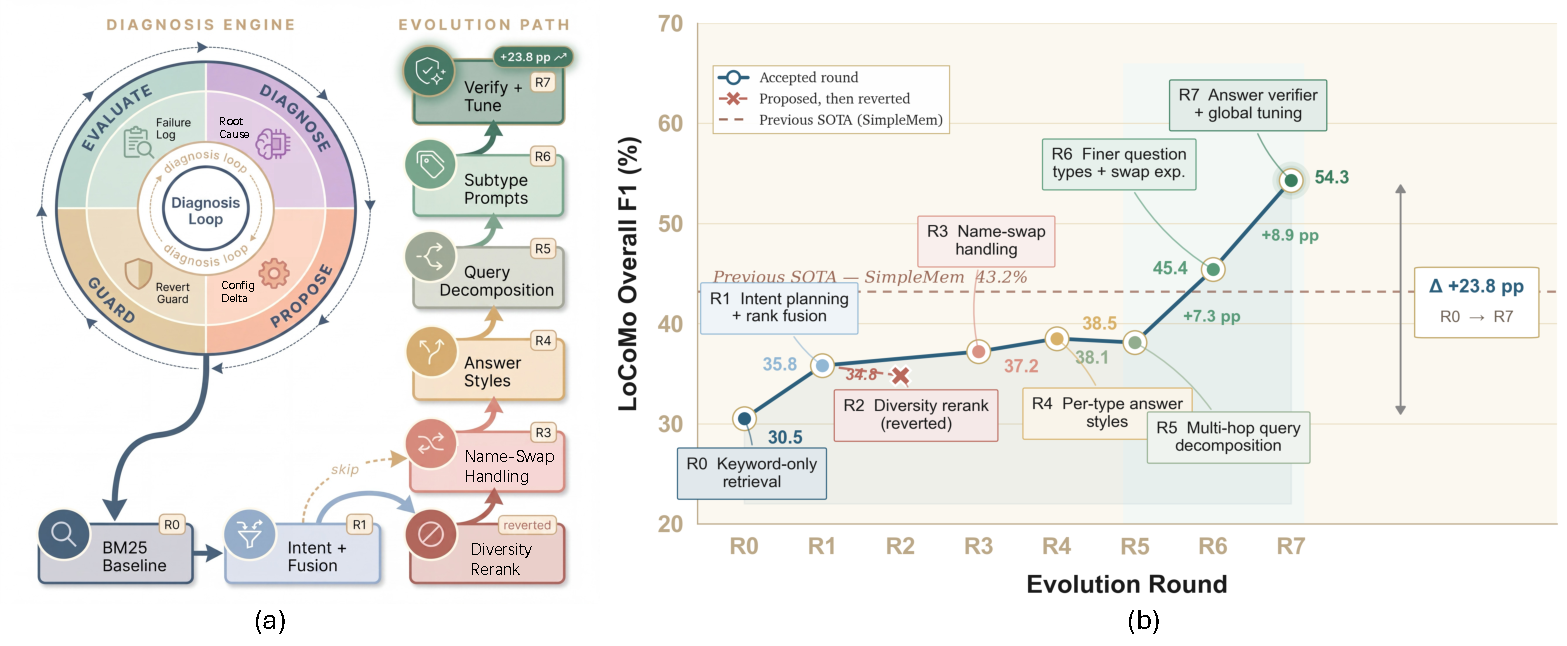
\includegraphics[width=\textwidth]{figs/traj_1.pdf}
    \caption{\textbf{\ours{} self-evolves its retrieval configuration on LoCoMo via AutoResearch.}
    \textbf{(a)} A four-step evolution loop (\textsc{Evaluate}--\textsc{Diagnose}--\textsc{Propose}--\textsc{Guard}) ratchets accepted proposals into the action space; harmful ones (e.g., R2) are auto-reverted.
    \textbf{(b)} Overall F1 trajectory (single-backbone GPT-4o): 30.5\% baseline to 54.3\% at R7.}
    \label{fig:teaser}
    \vspace{-1.5em}
\end{figure}

This assumption creates a mismatch that worsens over time. As stored memories grow from dozens to hundreds of heterogeneous records, a retrieval policy calibrated for the small store becomes suboptimal, and different question categories require fundamentally different retrieval strategies. Our key observation is that a truly adaptive memory system must evolve at two levels: the stored knowledge must be maintained and consolidated, and the retrieval infrastructure itself must self-adapt to the changing memory landscape and query distribution. Achieving such self-adaptation requires the system to autonomously observe its own failures, hypothesize root causes, test configuration changes, and retain only those that improve performance.

We present \ours{}, a memory architecture that autonomously evolves its retrieval infrastructure through LLM-driven closed-loop diagnosis. \ours{} combines a typed knowledge store with a multi-view retriever covering lexical, semantic, and structured-metadata signals, and exposes the complete retrieval configuration as a structured action space. An LLM-powered diagnosis module reads per-question failure logs, categorizes root causes, and proposes targeted configuration adjustments that a guarded meta-analyzer applies with automatic revert-on-regression safeguards. This closed-loop self-evolution constitutes an AutoResearch process: the system autonomously conducts the observe-hypothesize-experiment-validate cycle that would otherwise require manual researcher effort, discovering effective retrieval policies including entirely new configuration dimensions not present in the original framework.

In summary, our primary contribution is \ours{}, the first memory framework that autonomously evolves its retrieval infrastructure through LLM-driven closed-loop diagnosis, realizing an AutoResearch process that replaces manual configuration tuning. On LoCoMo, \ours{} outperforms the strongest published baseline by 25.7\% relative (78.0\% over the minimal baseline); on MemBench, it exceeds the strongest baseline by 18.9\% relative. The evolved configurations transfer across benchmarks with positive rather than catastrophic transfer.
